
\section*{\textbf{\underline{Abstract}}}
A central goal of ecology is to understand spatial patterns of species densities. Habitat suitability estimates from species distribution models (SDMs) could be used to represent species density and overcome the scarcity of density data. However, there is mixed evidence that habitat suitability relates to density, and it is suggested that local dynamics affect the relationship between habitat suitability and density. We simulated population dynamics for 200 virtual species with different combinations of factors (demographic stochasticity, dispersal, and intraspecific competition) that affect population sizes and trained SDMs considering different sets of environmental predictors to evaluate when habitat suitability reflected densities. We found that even when population growth rate and demographic stochasticity are the only factors driving population dynamics habitat suitability was not consistently related to species densities. Incorporating dispersal dynamics and spatial differences in intraspecific competition had small negative effects on the relationship between habitat suitability and density, showing that these factors influence these relationships. Species differences partially explained the variability in the relationship between habitat suitability and density across species. Similar results were found for 200 North American bird species, indicating that habitat suitability estimates from SDMs should not be used to understand species densities.

%-----------------------
\section*{\textbf{\underline{Introduction}}}
%\section*{Introduction}

The fundamental niche is a persistence threshold that defines the sets of environmental conditions that allows species to persist across geographic space \parencite{hutchinson1957,pulliam2000, colwell2009}. Several statistical methods that relate species occurrence data with environmental conditions have been developed to identify areas that are environmentally suitable for species occurrence \parencite{peterson2011}. These tools, frequently referred to as species distribution models (SDMs), are primarily used to estimate species geographic distributions and have been essential for answering macroecological and biogeographical questions as well as to aid conservation efforts \parencite{cayuela2009, calabrese2014,biber2020}. SDMs generate habitat suitability estimates where higher values represent more favorable conditions for species to occupy. These favorable conditions are usually assumed to support larger population sizes because of an increased survival and reproductive success of individuals occurring in these areas \parencite{weber2017,dallas2018,lee2022}, leading to a potential positive relationship between habitat suitability and species abundance \parencite{gomes2018}. In this case, \textit{density} (number of individuals per area) is perhaps the more appropriate term than abundance, as oftentimes it is the only possible measure. 


\paragraph*{}
This putative relationship between habitat suitability and density has spurred an interest in using SDMs to predict species densities \parencite{oliver2012sdm,acevedo2017,corbel2023}. Estimating species density through sampling approaches is a difficult task, such that a lack of spatial and temporal density data, a shortcoming called the \textit{Prestonian shortfall}, represents a major knowledge gap for most species \parencite{hortal2015}. Addressing this knowledge gap is important given that having information on species densities is crucial for understanding population dynamics. Using SDMs to predict species density is thus compelling given the more widespread availability of presence data that are often used in these models \parencite{pearce2006, bradley2016}. However, current evidence indicates that SDMs have limited efficacy in describing species density as most successful predictions come from cases where these relationships were assessed for single species whereas evaluations considering multiple species tend to be unsuccessful \parencite{weber2017,dallas2018,lee2022, waldock2022}.



\paragraph*{}
A lack of connection between habitat suitability and density could occur because a species density in a given location is affected by factors that are often ignored in SDMs \parencite{boulangeat2012}. For example, spatial differences in the level of intraspecific competition, because of differences in resource availability, can lead to complex spatial patterns of population dynamics \parencite{klomp1964, turnbull2007, zhang2021}. Dispersal can further affect observed population densities by allowing the persistence of populations in unsuitable environments through source-sink dynamics \parencite{pulliam1988,pulliam2000,furrer2016}. Moreover, when there are spatial differences in population growth rates and in intraspecific competition, dispersal can enhance population sizes and lead to larger than expected populations \parencite{oksanen1990,zhang2021}. When population sizes are small, demographic stochasticity plays an important role in driving population dynamics where these populations can face a higher extinction risk \parencite{gabriel1992,melbourne2008}. Since SDMs are trained on binary data and assume equilibrial dynamics, it can be particularly challenging for habitat suitability estimates to relate to species densities given the several factors, such as the ones outlined above, that affect population sizes.  
 
 

\paragraph*{}
Species tolerate different ranges of environmental conditions and use different types of resource, which could further lead habitat suitability estimates to be unrelated to density. For example, abundance-occupancy relationships describe the tendency for widespread species to be more locally abundant than restricted species, possibly because these widespread species are more generalist in terms of environmental conditions they tolerate or in the resources they use \parencite{borregaard2010,ten2022}. For such generalist species, SDMs might not be able to detect important environmental variables that limit their distributions, making these models unable to differentiate suitable and unsuitable environments in these cases \parencite{hernandez2006, van2016, harisena2021}. Conversely, species with restricted distributions can still achieve high densities in locations they occupy depending on local resource availability \parencite{komonen2009, crisfield2024}. As species might exhibit different types of specialization that can lead to complex patterns of geographic distributions and densities \parencite{crisfield2024}, SDMs might have difficulties distinguishing these types of specialization from occurrence data. Lastly, species can have performance curves (i.e., the relationship between how population growth rate changes along environmental conditions) with different characteristics that SDMs might also not be able to properly describe from occurrence data, which would ultimately render these models inappropriate for understanding densities \parencite{lee2022}.
 
\paragraph*{}
Here, we used a simulation framework to examine the effects of incorporating demographic stochasticity, dispersal, and intraspecific competition when modeling population dynamics across geographic space on the relationship between habitat suitability and density (Figure \ref{fig:conce_sdmabnd}). Simulated species had performance curves of different shapes and breadth to consider how species differences affect these relationships. To examine the generalities of these relationships in nature we also assessed how habitat suitability related to the density of 200 North American bird species. We found that habitat suitability was often positively correlated to density, but these relationships were highly variable and habitat suitability often explained $\approx 25\%$ and $\approx 5\%$ virtual species and North American birds densities, respectively. Demographic stochasticity, dispersal, and intraspecific competition had small negative effects on these relationships, and species differences and characteristics of the SDMs explained a small amount of the variability in these relationships across virtual species, suggesting that habitat suitability often does not reflect species densities.
 
%-----------------------
\section*{\textbf{\underline{Methods}}}
%\section*{Methods}
\paragraph*{Virtual species population dynamics}\mbox{}\\
We simulated 200 virtual species occurring in a lattice representing the United States and Canada (spatial resolution of 20 minutes that had 25207 cells, Figure \ref{fig:NA_prec}) using population models that considered different factors that influence population dynamics (Figure \ref{fig:conce_sdmabnd}). A discrete time Ricker model was used to simulate population dynamics, where populations grew according to population growth rate $R$ and intraspecific competition ($\alpha = 0.005$) limited population sizes. The number of offspring was treated as a Poisson random variable with mean of \textit{R} offspring per individual and survivorship was treated as a Binomial random variable with probability $e^{- \alpha N_{t}}$, representing the effects of demographic stochasticity in our model. 

\begin{equation}
\label{eq:ricker}
N_{t+1} = N_{t} \ R \ e^{- \alpha N_{t}}
\end{equation}  

In this model demographic stochasticity and population growth rate were the only factors causing changes in population sizes across generations. This model was expanded to also allow the occurrence of dispersal events between populations following a binomial random variable with probability $d$ ($d = 0.20$). Individuals dispersing from a focal population immigrated to new populations according to a negative exponential dispersal kernel \parencite{nathan2012} that was species-specific (Figure \ref{fig:kernel}). The maximum dispersing distance (in number of cells) was randomly chosen between 5 and 25 and the mean dispersal distance was a randomly chosen fraction between 0.1 and 0.6 of the maximum dispersal distance. Individuals could not disperse to cells outside the borders of the lattice (Figure \ref{fig:kern_crop}). This model was further expanded to allow spatial variation in the strength of intraspecific competition \parencite{zhang2021}. We used data on productivity to inform the intensity of intraspecific competition as productivity limits population and community sizes of several taxa \parencite{srivastava1998,cerezer2021}. We assumed a linear negative relationship between the productivity of a site and the level of intraspecific competition that a given population experienced ($\alpha = 0.005 - 0.1$). We used the normalized difference vegetation index (NDVI) as a proxy for productivity and we obtained NDVI data for the first day of June of 2020 from MODIS through the R package \texttt{MODIStsp} \parencite{busetto2016}. 

For each species, populations were simulated considering the following combination of factors: demographic stochasticity (considered our baseline model), demographic stochasticity and spatial intraspecific competition, demographic stochasticity and dispersal, and  demographic stochasticity, spatial intraspecific competition, and dispersal, resulting in four population simulations per species. Simulations started with all cells in the lattice occupied with 20 individuals from a given species and models ran for a total of 100 generations to allow population dynamics to reach equilibrium. By the end of the simulations, occupancy (fraction of occupied cells in the lattice) varied across species (0.38 $\pm$ 0.16), and we sampled 100-750 of those occupied cells to model the distribution of virtual species. We chose this number of cells for the virtual species to be consistent with the number of sites that the North American bird species considered in our study occupied (see below).   
 
Two performance curves, a symmetric and an asymmetric, were simulated for each virtual species considering mean annual temperature in the United States and Canada (see details in the \textit{Environmental predictors and model structure} section below). We simulated performance curves considering mean annual temperature because there is significant spatial variation in temperature patterns in North America (Figure \ref{fig:NA_prec}). Mean annual temperature values ranged $-$26$^{\circ}$C to 24.4 $^{\circ}$C, allowing the possibility of simulating species that tolerate different ranges of temperatures. Symmetric and asymmetric performance curves were used because several species have performance curves with these properties \parencite{oksanen2002, vasseur2014}. These performance curves represent how species' population growth rates change along temperature gradients, and they were used to estimate \textit{R} of each population occurring in a given location. We used the \textit{sech} function available in the \texttt{senlm} package \parencite{anderson2022} to simulate symmetric and asymmetric performance curves. A species had the same optimum temperature (location of the maximum, $m$ parameter in \textit{sech}) for both performance curves, and this optimum was randomly sampled between -15 and 14. However, curves differed in skewness (symmetry, $r$, parameter), where the skewness of the symmetric and asymmetric curves was  0 and -0.95, respectively. A negative value of skewness makes the performance curve have a broader left-hand tail while a value of 0 makes the performance curve symmetric \parencite{anderson2022}. Peakedness (peakedness, $p$, parameter) was chosen to be 3 and 5.25 for symmetric and asymmetric curves, respectively. The peakedness parameter controls the kurtosis of the performance curve and smaller values lead to flatter curves where population growth rates decrease more slowly away from the optimum environmental condition. Lastly, the spread (spread, $s$, parameter) of the asymmetric curves was $1/3$ of the spread of symmetric curves. The spread represents the range of temperature values that a species could tolerate, and these values were randomly sampled between 3 and 10. Our goal was to evaluate whether the shape and the breadth of a species performance curve could affect the relationship between habitat suitability and density. Figure \ref{fig:curves} shows an example of how a symmetric and an asymmetric performance curves change along the temperature gradient for a species. 

\paragraph*{North American bird density data}\mbox{}\\
We used data on North American bird species to compare habitat suitability estimates from SDMs to the density of these species to explore the generality of these relationships for real species. Bird density data were obtained from the Breeding Bird Survey (BBS; \textcite{sauer2020}). The BBS is a yearly standardized census of North American bird species that is performed by volunteers during the breeding season. In these surveys, routes of $\approx$ 50km are sampled every 1km for about three minutes through point counts where all birds seen or heard within a radius of 0.4 km are recorded. We used the data sampled from 1997-2019 to estimate the mean annual density and to model the distribution of 200 bird species that were observed occurring in 100-750 locations. We chose this temporal extent to calculate mean annual density because a consistent number of sites ($\approx$ 3000) have been continuously sampled by BBS since 1997, providing reliable estimates of population density for this time period. Incomplete sampling and detection probability could affect where species are recorded and their observed density and potentially influence the analyses of such data. However, incomplete sampling should not affect our study given the standardized nature of how the BBS data are collected, and also because there is limited evidence for potential biases influencing analyses of the BBS data across large spatial and temporal scales considering several species \parencite{rosenberg2019}. Moreover, the effects of detection probability are more prevalent when population sizes are small \parencite{tanadini2011, bennett2024}, such that both occurrence (used in SDMs to estimate habitat suitability) and density (used to relate to habitat suitability) data would be similarly affected by detection probability in these cases. This suggests that incomplete sampling or detection probability should have not influenced the relationship between habitat suitability and density that we observed for North American birds.

\paragraph*{Environmental predictors and model structure}\mbox{}\\
We obtained the 19 bioclimatic variables available in WorldClim 2.1 at a resolution of 10 minutes through the \texttt{geodata} R package \parencite{fick2017, geodata}. These variables include different measurements of temperature and precipitation patterns that are considered important determinants of species distributions \parencite{barbet2014, illan2014}. For the North American bird species, we performed a PCA over the 19 bioclimatic variables covering North America and used the first four axes as predictors to model the species distributions given that they explained over 90\% of the variation in the data \parencite{kriticos2014}. These environmental predictors were aggregated to have a resolution of 30 minutes when modeling the distribution of North American birds to match the spatial resolution in which the BBS data is sampled.  

The distribution of virtual species were modeled using different sets of environmental predictors. First, we modeled their distributions using mean annual temperature and NDVI as predictors. This represents a situation where there is a perfect knowledge about the environmental conditions that affect the population dynamics of species. SDMs were fitted using NDVI and mean mean annual temperature as predictors for the four population models that we considered. We also modeled species distributions using mean annual temperature, mean diurnal range in temperature, temperature seasonality, annual precipitation, precipitation of the wettest month, and precipitation seasonality (hereafter multiple environmental predictors). This exemplifies a situation where there is some knowledge about what variables potentially affect population dynamics, but unimportant predictors are also considered in the model. SDMs using these multiple environmental predictors were fitted for population models that simultaneously considered demographic stochasticity, spatial intraspecific competition, and dispersal. Lastly, we performed a principal components analysis (PCA) over these 19 bioclimatic variables covering the United States and Canada and used the first four axes that explained over 90\% of the variance of the data as predictors in the model. This constitutes a case where there is limited or no knowledge about the environmental factors that affect the population dynamics of a given species. SDMs using these PCA axes as predictors were also fitted for population models that simultaneously considered demographic stochasticity, spatial intraspecific competition, and dispersal. Thus, we were able to examine whether SDMs trained with uninformative environmental predictors had habitat suitability estimates that were less related to density. Environmental variables were aggregated to have a spatial resolution of 20 minutes when modeling the distribution of the virtual species to match the resolution in which their population dynamics were simulated. 

\paragraph*{Modeling and evaluating species distributions}\mbox{}\\
The distribution of virtual and real species was modeled using MaxEnt, a widely used machine-learning method that requires presence and pseudo-absence data and that generally have good performance \parencite{elith2010, santini2021}. Models were fit using default regularization coefficient values as these have been shown to perform well for a wide range of species and because fine tuning models individually for each species is impractical when considering several species as in our case \parencite{phillips2008, merow2013}. Prevalence of presences and pseudo-absences was kept at 0.5, where 50\% of the data used are presences and 50\% are pseudo-absences \parencite{senay2013, iturbide2015}. Pseudo-absences were randomly sampled from a 400km buffer surrounding presence points of virtual and real species. We used a cross-validation procedure, where 75\% of our dataset was used to train the models and the other 25\% was used to test the models. This process was repeated 20 times to account for potential differences in the habitat suitability estimates that could arise from using specific sets of presences and pseudo-absences when training and testing the models. Models were evaluated using the area under the receiver operating characteristic curve (AUC) \parencite{fielding1997}. AUC is a discrimination performance measure that assesses how well a model distinguishes between presences and pseudo-absences, where values closer to 1 suggests a model is good at differentiating presences from pseudo-absences and values around 0.5 indicates a random performance. Habitat suitability estimates and AUC were averaged across species considering the 20 models that were fitted for each species. For the virtual species, we assessed whether habitat suitability estimates produced by SDMs could replicate their performance curves. Performance curves were rescaled to 0-1 and we compared, along the temperature gradient, the difference between observed mean habitat suitability produced by SDMs and the actual population growth rate in a given environment based on the performance curve of the species.




\paragraph*{Assessing the relationship between habitat suitability and density}\mbox{}\\
The presence data used to model species distributions were used to evaluate how habitat suitability related to species density.  We extracted habitat suitability for each presence point, and we used the observed population size to represent species densities in those locations. The relationship between habitat suitability and density was evaluated using Pearson's correlations. To examine how well habitat suitability explained density, we calculated the coefficient of determination, which is equal to the squared Pearson's correlation coefficient. 

We fitted two linear mixed-effect models to evaluate the effects of different factors on the relationship between habitat suitability and density across species. In both LMMs, we used the correlation coefficient ($r$) between habitat suitability and density as the response variable and species were used as random effects, but different fixed effects were considered. In our first LMM, our goal was to understand how factors that contribute to local population dynamics affect the relationship between habitat suitability and density. We encoded dummy variables to assess how considering dispersal and spatial intraspecific competition in population models affected these relationships. Demographic stochasticity was present in all models and was considered our baseline case. Thus, we did not encode a dummy variable for demographic stochasticity. In this LMM, we also considered whether using multiple environmental predictors or PCA axes when training SDMs affected the relationship between habitat suitability and density by encoding dummy variables for these predictors. In our second LMM, we were interested in understanding how species differences and SDMs characteristics could affect the relationship between habitat suitability and density. Fixed effects considered were the breadth and the shape (i.e., symmetric or asymmetric) of species performance curves, the mean absolute difference between habitat suitability and population growth rate (estimated from presences), and the mean SDM performance. In this model, continuous predictors were in different scales and they were standardized to allow comparisons of their effects on the relationship between habitat suitability and density. LMMs were fit using the \texttt{glmmTMB} R package \parencite{brooks2017} while model diagnostics (models assumptions were genrally met; see Figures \ref{fig:mod_dyn}-\ref{fig:mod_sp} and Appendix B for details) and goodness of fit (Nakagawa's conditional $R^2$) were estimated using the \texttt{performance} R package \parencite{ludecke2021}. This conditional $R^2$ takes fixed and random effects into account when estimating the model goodness of fit. 
%-----------------------
\section*{\textbf{\underline{Results}}}
%\section*{Results}


\paragraph*{Do demographic stochasticity, dispersal, and intraspecific competition affect the relationship between habitat suitability and density?}\mbox{}\\
Correlations between habitat suitability and density were often significant and positive, but the strength of these relationships varied considerably across species within the different models of population dynamics (Figure \ref{fig:cor}a), and habitat suitability explained $\approx$ 25\% of the variation in species density (Figure \ref{fig:cor}b). Habitat suitability was not consistently related to density even when population dynamics were driven solely by population growth rates and demographic stochasticity and SDMs were trained with the two environmental factors that affected the density of species. We found that in the baseline case (the intercept) of our first LMM, the average correlation between habitat suitability and density was 0.48. This correlation is reduced to 0.45 for population models that considered dispersal ($\beta = -0.027$, $p < 0.01$) and to 0.41 for models that considered spatial differences in intraspecific competition ($\beta = -0.069$, $p < 0.01$; Figure \ref{fig:cor}c). Nakagawa's conditional $R^2$ was 0.28, indicating that this LMM had a relatively limited explanatory power. The performance of SDMs widely varied across virtual species, such that these models tended to have lower performance for species that have broader performance curves (see Appendix B and Figure \ref{fig:auc}).


SDMs were more consistently able to identify the important environmental predictor that drives population growth rate when they were trained with mean annual temperature and NDVI than when multiple environmental predictors were considered (Figure \ref{fig:imp}). However, using multiple environmental predictors had no effect on the correlation between habitat suitability and density, while using PCA axes as predictors negatively affected these relationships ($\beta = -0.099$, $p < 0.01$; Figure \ref{fig:cor}c). This suggests that having no information on environmental factors that affect population dynamics may lead to habitat suitability estimates that are less related to species densities.


\paragraph*{What explains the high variability in the relationship between habitat suitability and density?}\mbox{}\\
We found that the high variability in the relationship between habitat suitability and density observed across virtual species could be explained by some of the factors that we considered in our second LMM. The baseline case (the intercept) of this LMM had an average correlation between habitat suitability and density of 0.39. Habitat suitability tended to relate less to the density of species that had broader performance curves ($\beta = -0.039$, $p < 0.01$; Figure \ref{fig:diff}a, e) or when habitat suitability poorly reflected population growth rates ($\beta = -0.061$, $p < 0.01$; Figure \ref{fig:diff}b, e). SDMs performance and the shape of species performance curves did not affect the relationship between habitat suitability and density (Figure \ref{fig:diff}c-e). Nakagawa's conditional $R^2$ was 0.20, also suggesting that this LMM could not explain most of the variation in the relationship between habitat suitability and density across species. 


\paragraph*{What is the relationship between habitat suitability and density for North American birds?}\mbox{}\\
We found that habitat suitability and density were positively correlated for 54\% of the North American birds, while negative and non-significant relationships were observed for 5.5\% and 40.5\% of the species, respectively (Figure \ref{fig:cor}a). Despite finding these positive relationships, habitat suitability rarely explained over $5\%$ of the variation in density of North American birds (Figure \ref{fig:cor}b). These results showed that habitat suitability is less often related to the density of real species compared to virtual species, and significant correlations could only explain a particularly small fraction of the variation in density of North American birds. Nevertheless, SDMs performed relatively well for North American birds (Figure \ref{fig:auc}). Overall, our results highlight a general disconnect between habitat suitability and species densities for virtual species and North American birds.








%-----------------------

\section*{\textbf{\underline{Discussion}}}
%\section*{Discussion}
We found that habitat suitability is often positively correlated to density, but these relationships were widely variable across species and had low explanatory power, indicating that habitat suitability estimates might be unreliable for understanding species densities. The disconnect between habitat suitability and density often reported for real species is usually attributed to the fact that several factors, such as dispersal dynamics or resource limitation, acting at the local scale could lead to complex spatial patterns of density that habitat suitability would be unable to capture \parencite{weber2017,dallas2018,jimenez2021}. We show that even when population growth rates and demographic stochasticity were the only factors influencing population sizes, habitat suitability estimates were still not consistently related to species densities. Incorporating dispersal dynamics and spatial intraspecific competition to our models had small negative effects on these relationships, showing that these factors influenced the relationship between habitat suitability and density. However, these findings also suggest that demography and dispersal may not be the main factors responsible for the weak link between habitat suitability and density. 

\paragraph*{}
The general disconnect between habitat suitability and density could occur because the presence data used to train SDMs might not contain the necessary information to describe densities. For example, high habitat suitability might suggest high probability of occurrence, but not of density, as environmental conditions can differently affect species occurrence and density \parencite{bradley2016}. SDMs that have poor performance and are unable to differentiate between presences and pseudo-absences are unlikely to be able to reflect densities altogether \parencite{jimenez2021}, but we observed that SDMs that had high performance did not produce habitat suitability estimates that were more closely related to density. This demonstrates that a model that is suitable for estimating occurrences does not necessarily translates into a model that is suitable for estimating densities. SDMs that produced habitat suitability estimates that more properly reflected population growth rates led to stronger correlations between habitat suitability and density across species. This occurs because these models provide a more accurate description of how species performances, and consequently the potential population size in a given area, change along environmental gradients. However, SDMs might be particularly unable to describe performance curves of species that tolerate a wide range of environmental conditions because these models often cannot discriminate suitable from unsuitable environments for such generalist species \parencite{hernandez2006,franklin2009,van2016}. This would explain why habitat suitability is less related to the density of species that have broader performance curves. 
 

\paragraph*{}
When assessed for a large number of mammals and plant species, the relationship between habitat suitability and density is often non-significant or is in contrasting directions \parencite{dallas2018,sporbert2020}. We also observed variable relationships between habitat suitability and density for the 200 North American birds species that we considered. The positive relationship between habitat suitability and density found for about half of the species we considered could be occurring because these birds might have higher dispersal ability and are more capable of tracking suitable environments across geographic space and over time \parencite{tingley2009, zurell2018}. This may occur through informed dispersal behavior where individuals would be more likely to disperse to good habitat patches \parencite{clobert2009, oro2021}. Alternatively, our simulations did not consider informed dispersal, which led to the occurrence of source-sink dynamics by allowing individuals to occupy unsuitable sites \parencite{pulliam1988, pulliam2000, furrer2016}. This could explain why dispersal had a negative effect on the relationship between habitat suitability and density of virtual species. Nonetheless, habitat suitability was still not able to explain most of the variation in the density of North American birds. This could be occurring because areas predicted to be of high environmental suitability can have populations of either low or high density \parencite{vanderwal2009, acevedo2017, braz2020}. Moreover, populations occurring in locations with low habitat suitability can still have positive growth rates \parencite{thuiller2014,cserg2017}, and potentially reach high densities, which could further obscure any potential relationship between habitat suitability and density. 


\paragraph*{}
Demographic stochasiticity, dispersal, and intraspecific competition affect local densities \parencite{melbourne2008,furrer2016, zhang2021}, but these factors seem to have played a limited role in driving the disconnect between habitat suitability and density in our simulations given their relatively small negative impacts on these relationships. However, it is likely that an interplay between different factors could lead to the general weaker, or lack of, relationship between habitat suitability estimates and density of real species. For example, interspecific competition and environmental stochasticity affect population densities \parencite{may1973, robertson1996} and could be interacting with the factors that we considered in our study to influence these relationships even more for real species \parencite{santini2019, braz2020}. The presence of sampling biases in the occurrence data that are often used to fit SDMs \parencite{inman2021,bowler2023}, alongside with the use of environmental conditions that might not be related to the population dynamics of species, such as PCA axes, may further increase the disconnect between habitat suitability and density for real species. 


\paragraph*{}
Using SDMs to predict species densities is compelling because the presence data used in these models are more readily available than density data \parencite{pearce2006, bradley2016, hortal2015}, but our findings suggest that SDMs should not be used for these purposes as they fail to describe different aspects of population dynamics under a wide range of scenarios. SDMs can still be useful for predicting species occurrences \parencite{lee2022}, but there is a growing body of evidence showing that their use to estimate densities should be avoided. Population densities in a given location is affected by a myriad of factors and using demographic models that are tailored specifically to predicting densities is a more productive path forward \parencite{dallas2018, lee2022}. Citizen-science databases that have count data could be used, for example, to test the predictions made by these demographic models and it could improve our understanding of population trends \parencite{dennis2017, fink2020}. 

\section*{\textbf{\underline{Figures}}}
%\section*{Figures}

\begin{figure}[ht]
\centering
\centerline{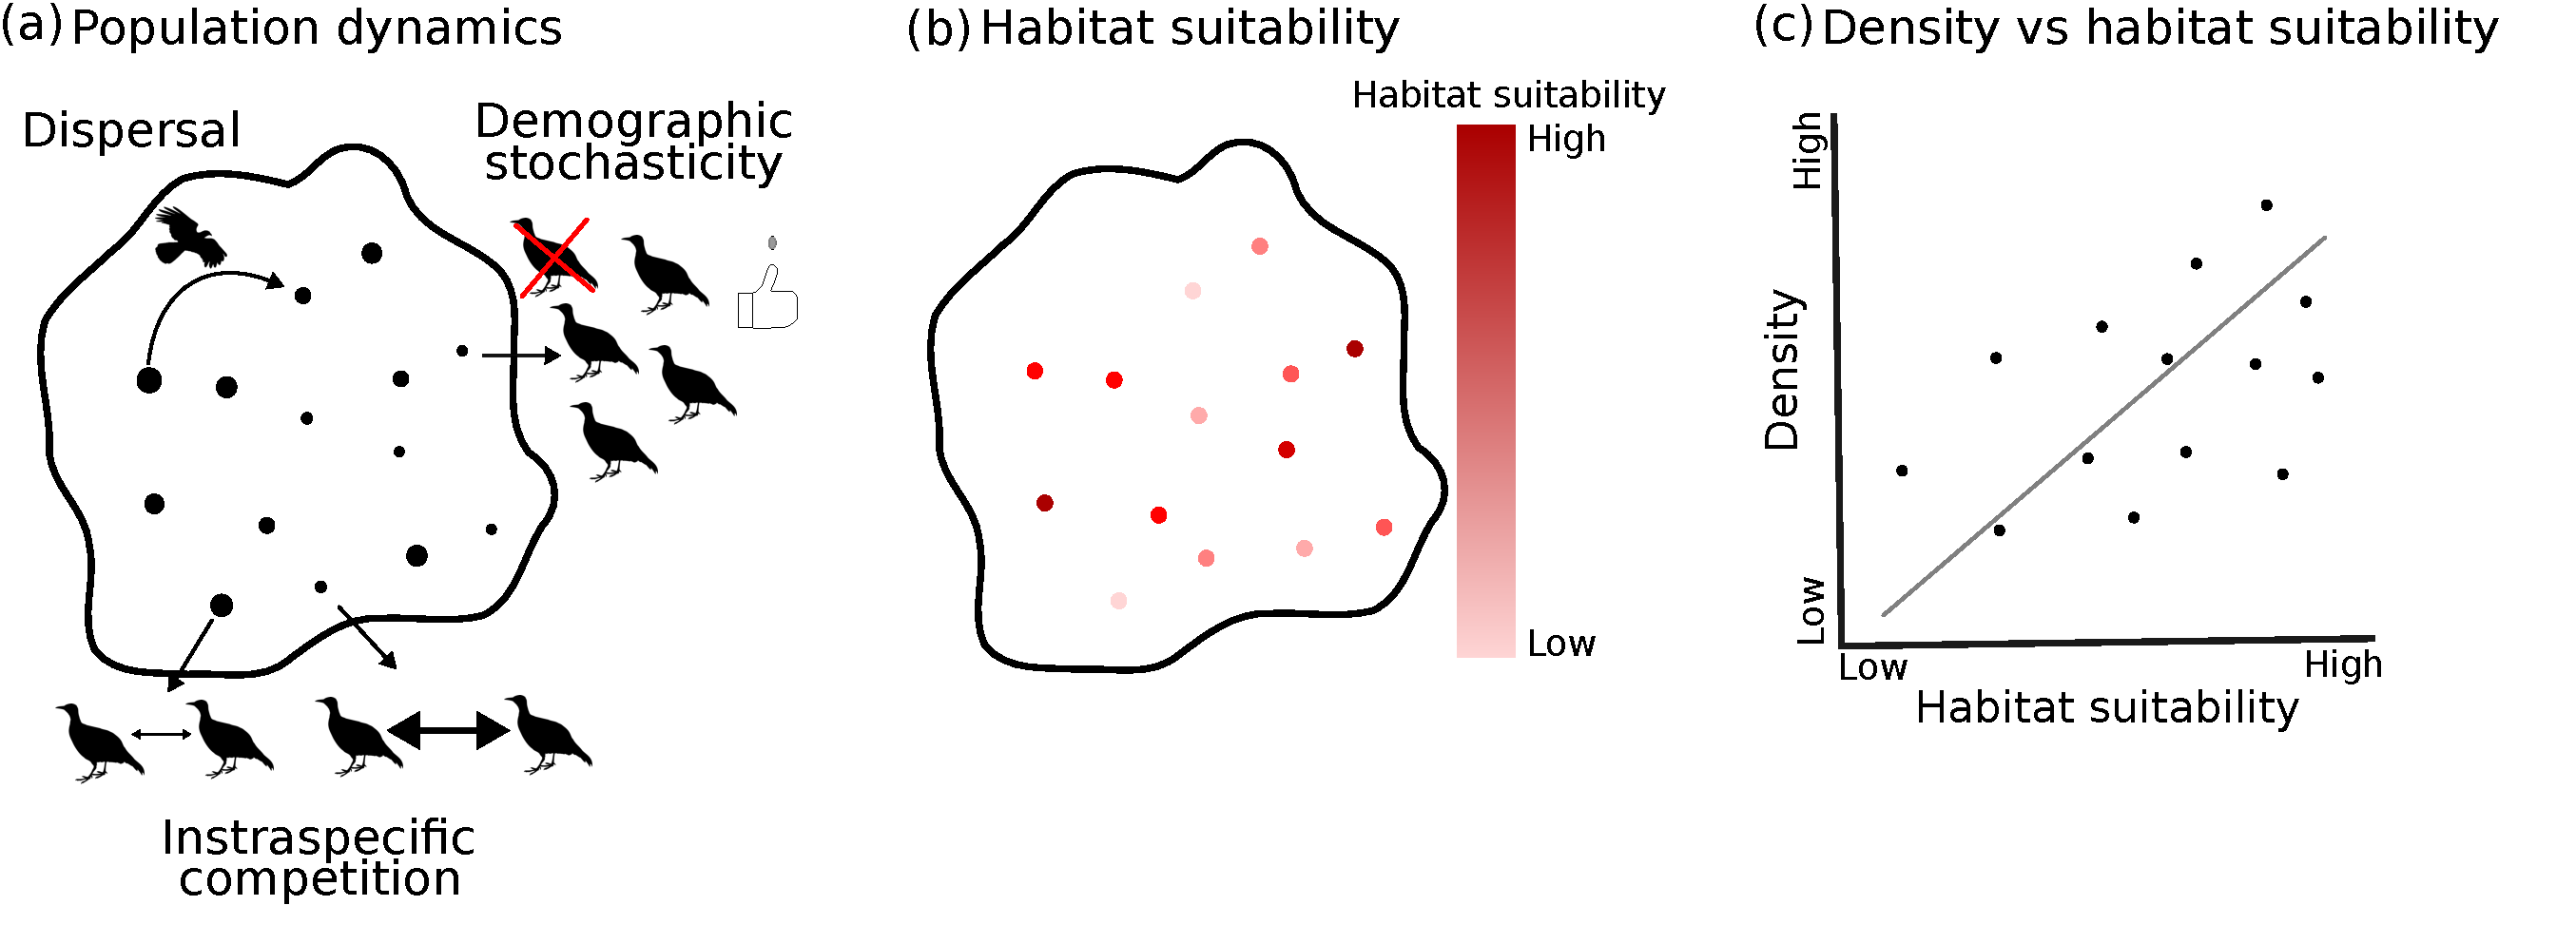
\includegraphics[width=1\textwidth]{FigsdmAbnd/Conceptual2}}
\caption[Simulating population dynamics]{Populations of virtual species were simulated considering dispersal dynamics, demographic stochasticity, spatial differences in intraspecific competition. Habitat suitability was estimated using species distribution models for sites were populations occurred (b) to explore the relationship (grey line) between habitat suitability and densities (c).} 
\label{fig:conce_sdmabnd}
\end{figure}
\clearpage

\begin{figure}[ht]
\centering
\centerline{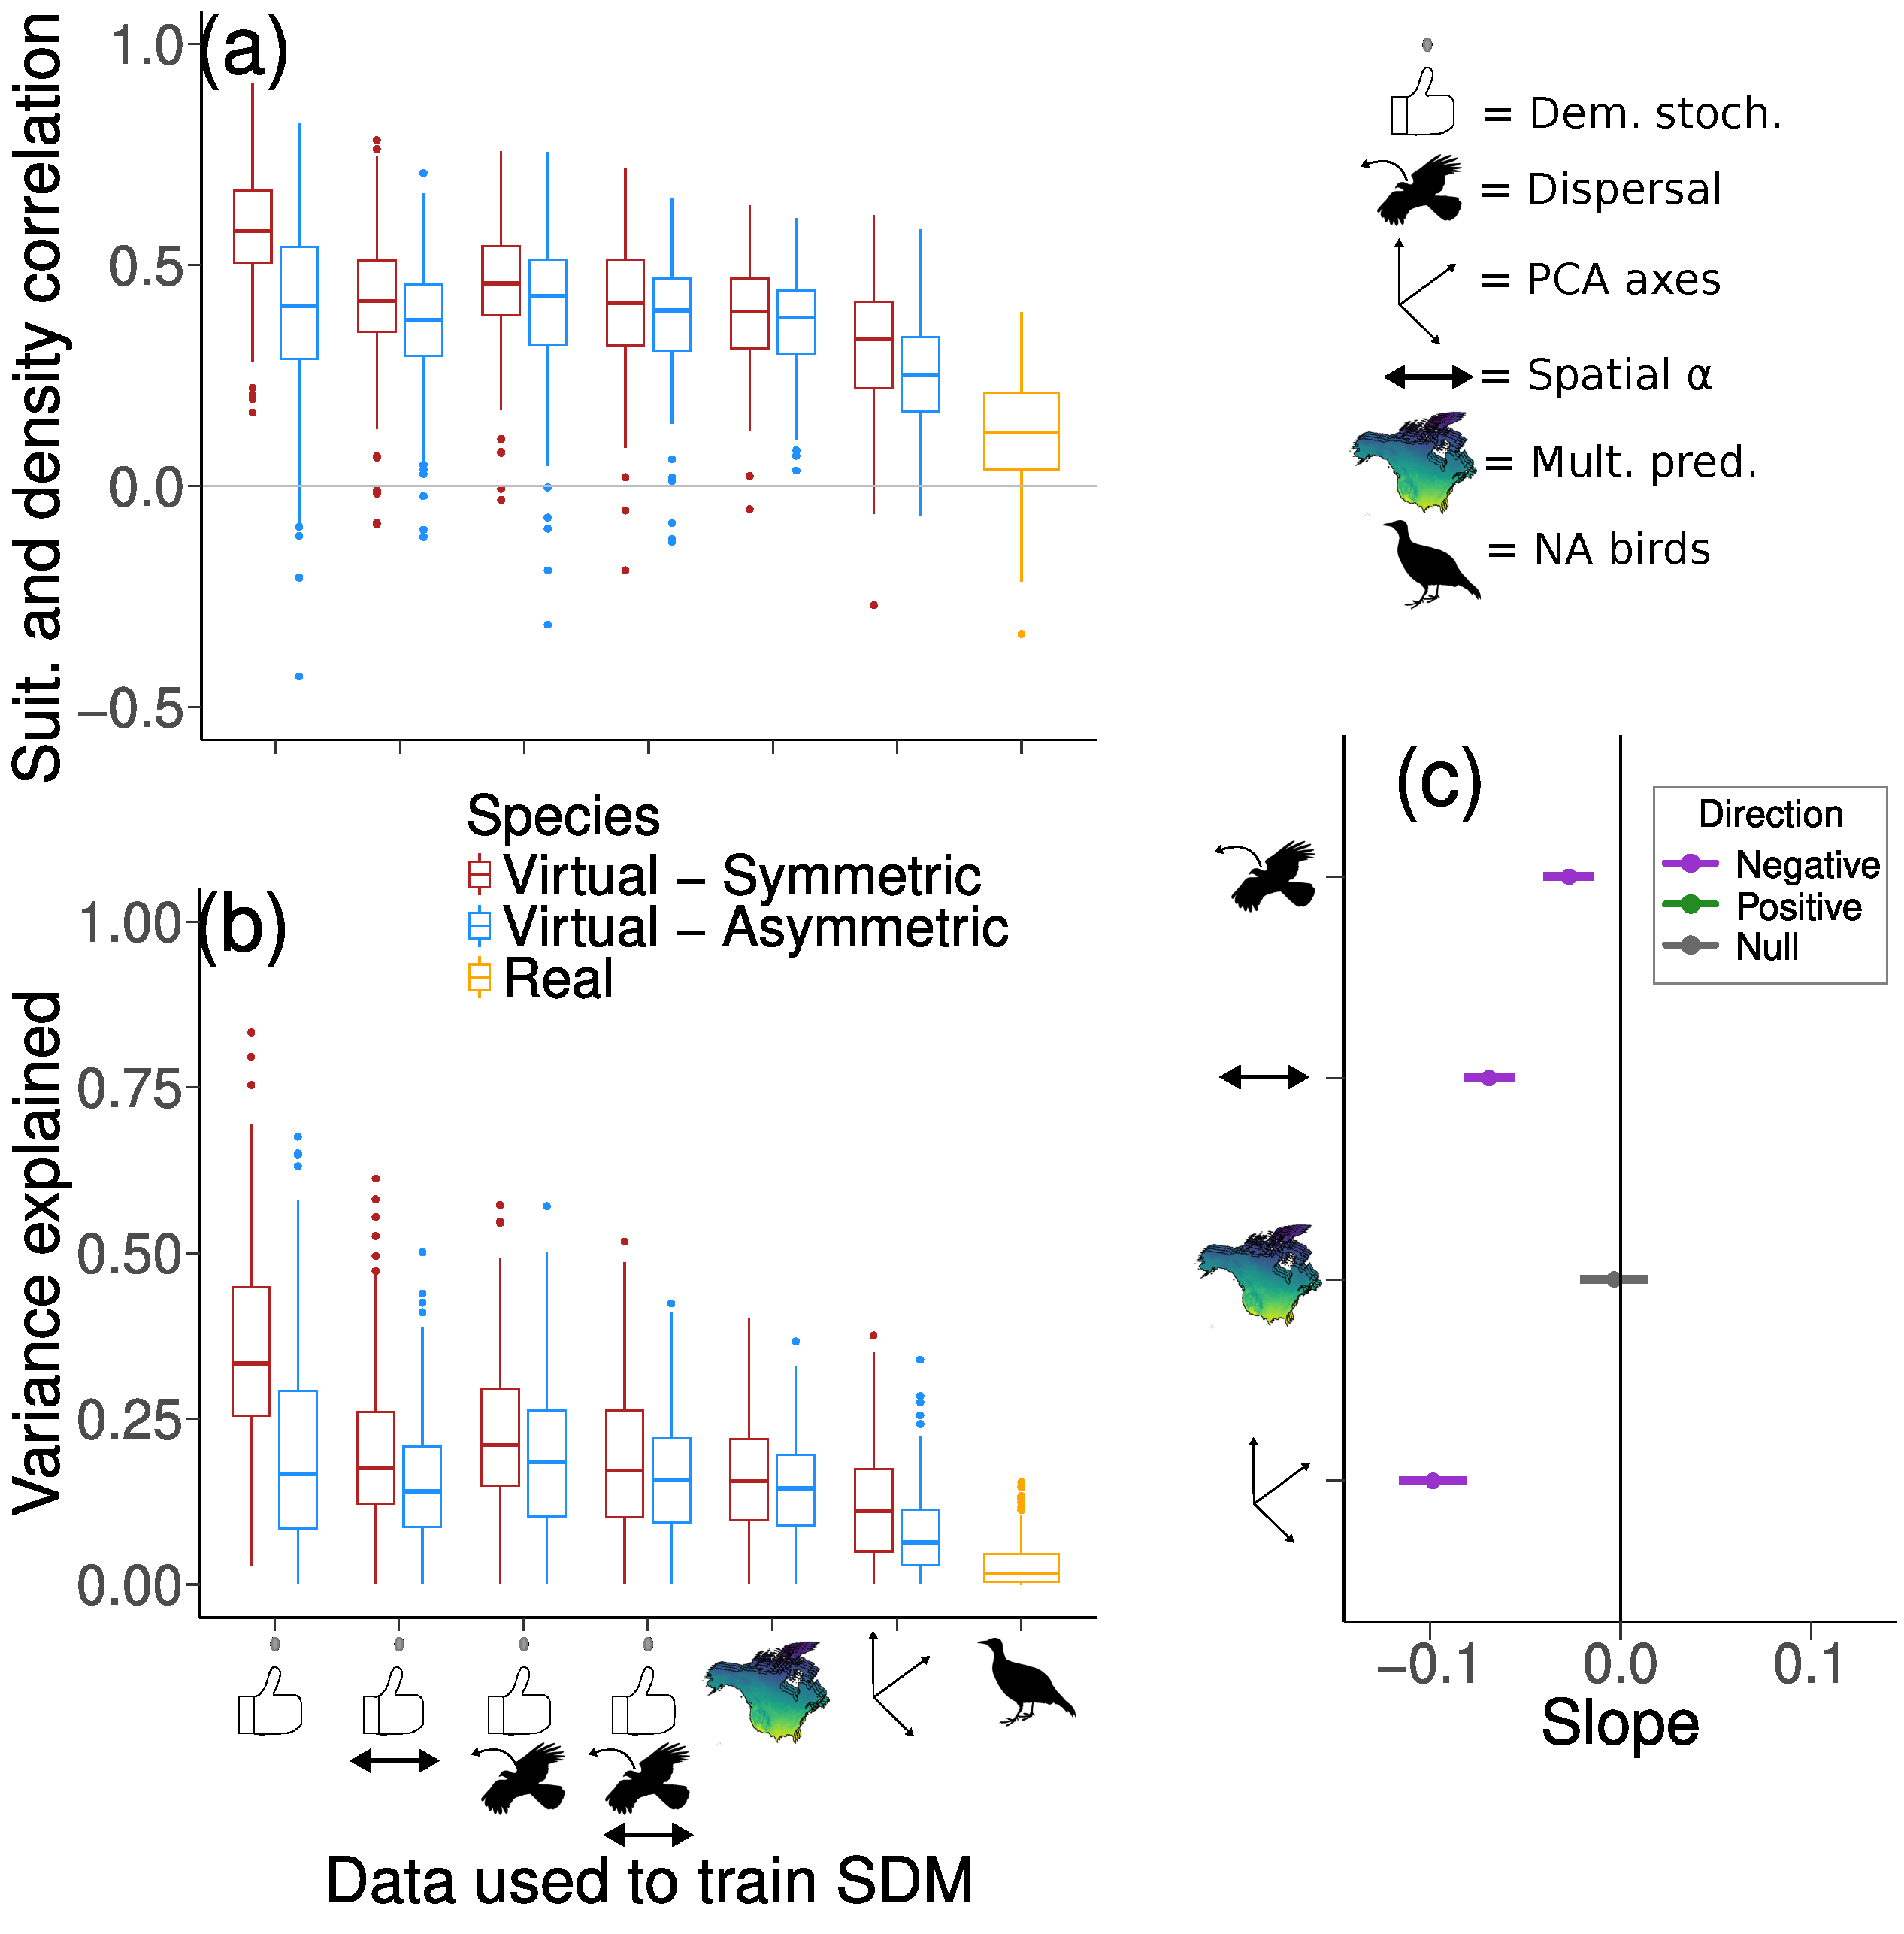
\includegraphics[width=1\textwidth]{FigsdmAbnd/Viores}}
\caption[Local factors influence how habitat suitability relates to density]{Observed correlations between habitat suitability and density for virtual species with symmetric and asymmetric performance curves and for North American birds.} 
\label{fig:cor}
\end{figure}
\clearpage


\begin{figure}[ht]
\centering
\centerline{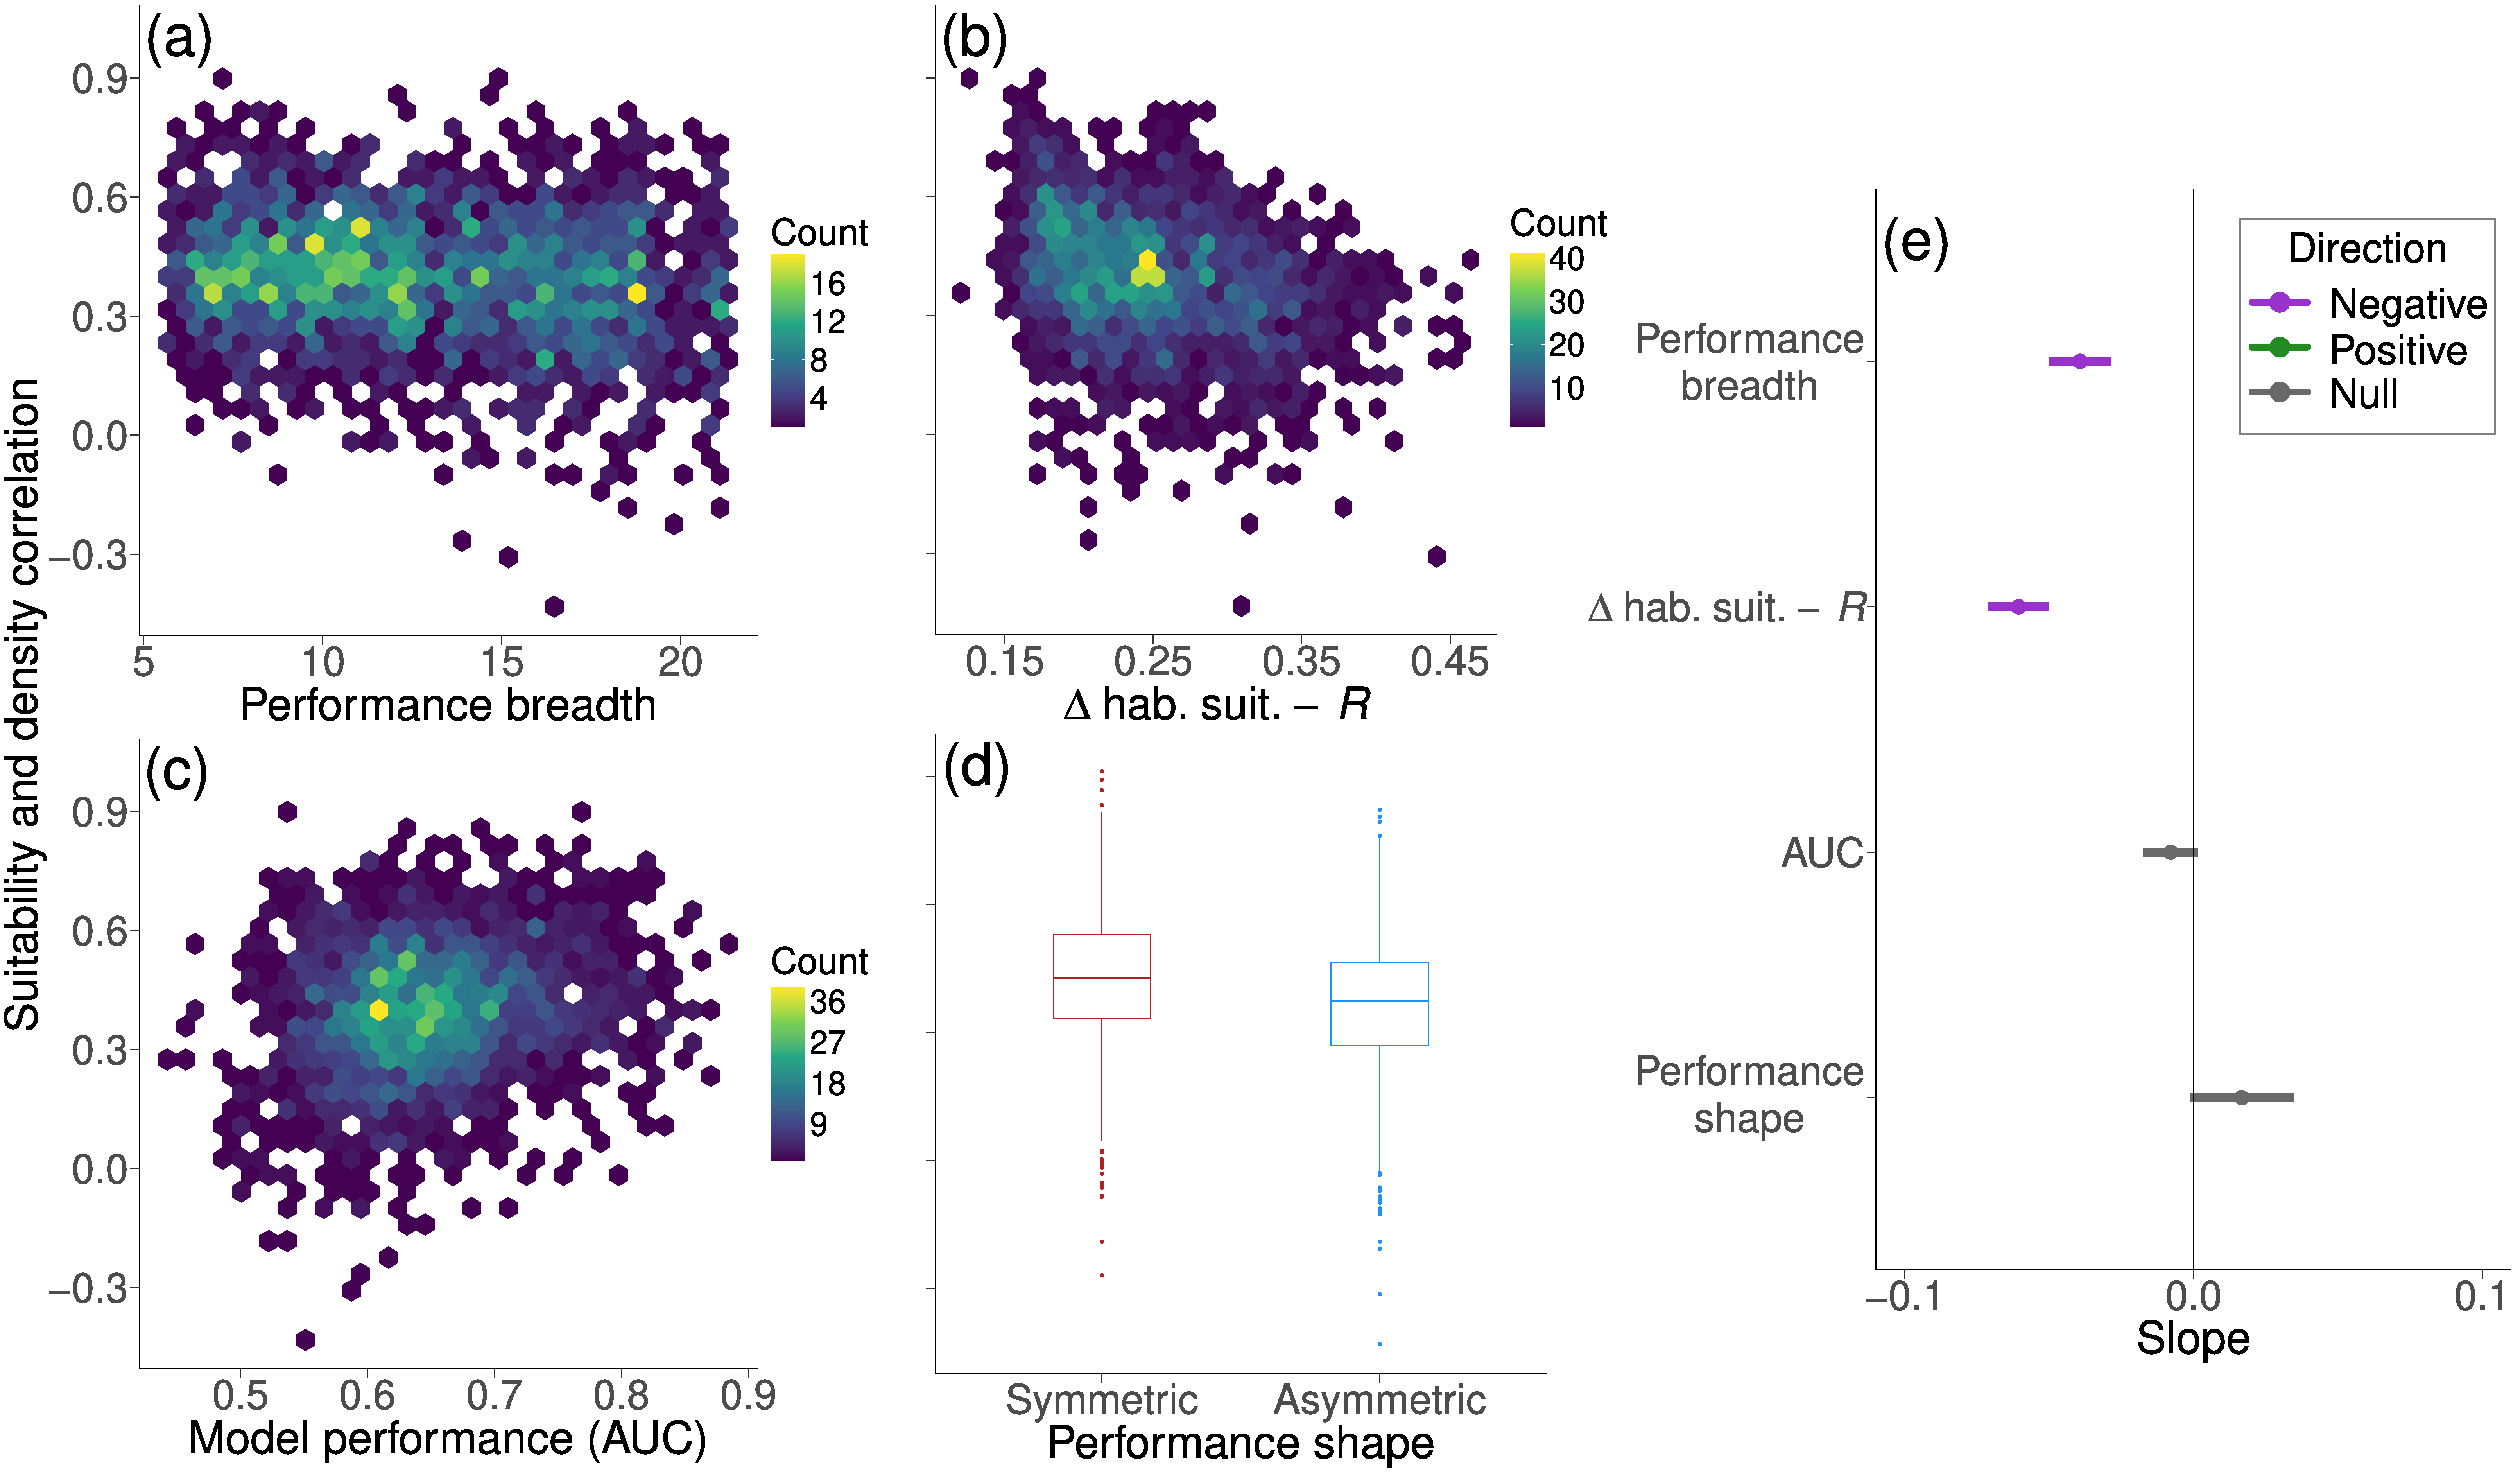
\includegraphics[width=1\textwidth]{FigsdmAbnd/RangeDiff}}
\caption[Species differences affect how habitat suitability relates to density]{The correlation between habitat suitability and density is affected by the species performance breadth, the ability of habitat suitability estimates to accurately represent population growth rates, but not by the average SDM performance and the shape of species performance curves.} 
\label{fig:diff}
\end{figure}
